\documentclass[main.tex,fontsize=8pt,paper=a4,paper=portrait,DIV=calc,]{scrartcl}
% Document
\usepackage[T1]{fontenc}
\usepackage[dvipsnames]{xcolor}
\usepackage[nswissgerman,english]{babel}
\renewcommand{\familydefault}{\sfdefault}

% Format
\usepackage[top=5mm,bottom=1mm,left=5mm,right=5mm]{geometry}
%\setlength{\headheight}{\baselineskip}
%\setlength{\headsep}{0mm}

%\usepackage{scrlayer-scrpage}
%\clearpairofpagestyles
%\chead{{\bfseries\TITLE, \AUTHOR, \pagename~\thepage}}

%\addtokomafont{pagehead}{\upshape}

\usepackage{multicol}
\setlength{\columnsep}{2mm}
\setlength{\columnseprule}{0.1pt}

% Math
\usepackage{amsmath}
\usepackage{amssymb}
\usepackage{amsfonts}

% Code
\usepackage{fancyvrb, etoolbox, listings, xcolor}
%\usemintedstyle{bw}

%\newminted[shell]{bash}{
%fontsize=\footnotesize,
%fontfamily=tt,
%breaklines=true,
%frame=single,
%framerule=0.1pt,
%framesep=2mm,
%tabsize=2
%}
%\newminted{css}{
%breaklines=true,
%tabsize=4,
%autogobble=true,
%escapeinside=||,
%stripall=true,
%stripnl=true,
%}

    \definecolor{lightgray}{rgb}{0.95, 0.95, 0.95}
    \definecolor{darkgray}{rgb}{0.4, 0.4, 0.4}
    \definecolor{purple}{rgb}{0.65, 0.12, 0.82}
    \definecolor{ocherCode}{rgb}{1, 0.5, 0} % #FF7F00 -> rgb(239, 169, 0)
    \definecolor{blueCode}{rgb}{0, 0, 0.93} % #0000EE -> rgb(0, 0, 238)
    \definecolor{greenCode}{rgb}{0, 0.6, 0} % #009900 -> rgb(0, 153, 0)
    \definecolor{teal}{rgb}{0.0, 0.5, 0.5}

\lstdefinestyle{code}{
    identifierstyle=\color{black},
    keywordstyle=\color{blue}\bfseries\small,
    ndkeywordstyle=\color{greenCode}\bfseries\small,
    stringstyle=\color{ocherCode}\ttfamily\small,
    commentstyle=\color{teal}\ttfamily\textit\small,
    basicstyle=\ttfamily\small,
    breakatwhitespace=false,         
    breaklines=true,                 
    captionpos=b,                    
    keepspaces=true,                 
    showspaces=false,                
    showstringspaces=false,
    showtabs=false,                  
    tabsize=2,
    belowskip=-5pt
}



% Images
\usepackage{graphicx}
\newcommand{\pic}{\includegraphics[scale=0.3]}
\graphicspath{{Screenshots/}{../Screenshots}}
\makeatletter
\def\pictext#1#2{%
    \@ifnextchar[{%
    \pictext@iiiii{#1}{#2}%
    }{%
      \pictext@iiiii{#1}{#2}[0.5,0.4,0.3]% Default is 5
    }%
}
\def\pictext@iiiii#1#2[#3,#4,#5]{\begin{minipage}{#3\textwidth}\includegraphics[scale=#4]{#1}\end{minipage}\begin{minipage}{#5\textwidth}#2\end{minipage}}
\def\minipg#1#2{%
    \@ifnextchar[{%
    \minipg@iiii{#1}{#2}%
    }{%
      \minipg@iiii{#1}{#2}[0.3,0.6]% Default is 5
    }%
}
\def\minipg@iiii#1#2[#3,#4]{\vspace{0.8mm}\begin{minipage}{#3\textwidth}#1\end{minipage}\begin{minipage}{#4\textwidth}#2\end{minipage}{\vspace{0.8mm}}}
\makeatother

%\newenvironment{minty}[2]% environment name
%{% begin code
%  \begin{minipage}{#1}
%  \begin{minted}{#2}
%}%
%{% end code
%  \end{minted}
%  \end{minipage}
%  \end{minty}\ignorespacesafterend
%} 

% Smaller Lists
\usepackage{enumitem}
\setlist[itemize,enumerate]{leftmargin=3mm, labelindent=0mm, labelwidth=1mm, labelsep=1mm, nosep}
\setlist[description]{leftmargin=0mm, nosep}
\setlength{\parindent}{0cm}

% Smaller Titles
\usepackage[explicit]{titlesec}

%% Color Boxes
\newcommand{\sectioncolor}[1]{\colorbox{black!60}{\parbox{0.989\linewidth}{\color{white}#1}}}
\newcommand{\subsectioncolor}[1]{\colorbox{black!50}{\parbox{0.989\linewidth}{\color{white}#1}}}
\newcommand{\subsubsectioncolor}[1]{\colorbox{black!40}{\parbox{0.989\linewidth}{\color{white}#1}}}
\newcommand{\paragraphcolor}[1]{\colorbox{black!30}{\parbox{0.989\linewidth}{\color{white}#1}}}
\newcommand{\subparagraphcolor}[1]{\colorbox{black!20}{\parbox{0.989\linewidth}{\color{white}#1}}}

%% Title Format
\titleformat{\section}{\vspace{0.5mm}\bfseries}{}{0mm}{\sectioncolor{\thesection~#1}}[{\vspace{0.5mm}}]
\titleformat{\subsection}{\vspace{0.5mm}\bfseries}{}{0mm}{\subsectioncolor{\thesubsection~#1}}[{\vspace{0.5mm}}]
\titleformat{\subsubsection}{\vspace{0.5mm}\bfseries}{}{0mm}{\subsubsectioncolor{\thesubsubsection~#1}}[{\vspace{0.5mm}}]
\titleformat{\paragraph}{\vspace{0.5mm}\bfseries}{}{0mm}{\paragraphcolor{\theparagraph~#1}}[{\vspace{0.5mm}}]
\titleformat{\subparagraph}{\vspace{0.5mm}\bfseries}{}{0mm}{\subparagraphcolor{\thesubparagraph~#1}}[{\vspace{0.5mm}}]

%% Title Spacing
\titlespacing{\section}{0mm}{0mm}{0mm}
\titlespacing{\subsection}{0mm}{0mm}{0mm}
\titlespacing{\subsubsection}{0mm}{0mm}{0mm}
\titlespacing{\paragraph}{0mm}{0mm}{0mm}
\titlespacing{\subparagraph}{0mm}{0mm}{0mm}

%% format cells
\usepackage[document]{ragged2e}
\usepackage{array, makecell}
\renewcommand{\arraystretch}{2}
\newcommand{\mc}{\makecell[{{m{1\linewidth}}}]}



\lstset{
    language=c++,
    style=code,
}
%%%%%

\begin{document}
\begin{table}[h!]
\section{Basic Terms and Information}
\begin{tabular}{|m{0.2\linewidth}|m{0.755\linewidth}|}
\hline
Preprocessor & Handles the \#include or \#def commands. Essentially loads these includes and places them where needed. Files after this stage have the .i notation -> main.i \\
\hline
Compiler & Turns the Code into an executable. Note that libraries are not automatically included here. Files after this stage have the .o notation -> main.o \\
\hline
Linker & Indluces the libraries at the end and puts them into the executable. This is used to run this binary on a pc without these libraries installed. Files after this stage no longer have a special notation. \\
\hline
\textbf{\emph{Declaration}}
&
This only declares the variable, it does not have a predefined value -> undefined behavior!\newline
\begin{lstlisting}
int i;
char c;
\end{lstlisting}
\\
\hline

\textbf{\emph{Definition}}
&
This defines a variable with a set value.\newline
\begin{lstlisting}
int i = 5;
int a{5};
\end{lstlisting} 
\, \newline
\textcolor{red}{\textbf{PLEASE, note the \emph{extern} keyword}}\newline
\textcolor{orange}{This means that only a tag is declared, there is no memory allocation yet.\newline
Without extern the memory is allocated, this is as the extern expects the variable to be declared/defined somewhere else}\\
\hline

\textbf{\emph{Variables close to usage}}
&
\pic{2022-09-27-08:41:06.png}\\
\hline
\end{tabular}
\subsection{Preprocessor Commands:}
\begin{tabular}{|m{0.2\linewidth}|m{0.755\linewidth}|}
\hline
\#ifdef / \#ifndef \newline \#define \newline \#endif & These are used to check if things are already defined, or to define them. Either for checks to avoid double definition, or to check if debug is used -> ifdef DEBUG\\
\hline
Include differences & \#include <library> \textcolor{teal}{search in the system include directories!}\newline
\#include "library" \textcolor{teal}{search in the current working directory, \textbf{AND after that in the system includes}}\\
\hline
\#pragma once & This is used to automatically avoid double include statements. Aka if it is included already simply ignore any double includes. \\
\hline
\textbf{Macros simple object version} & 
\#define XYZ 123 \newline
int x = XYZ compiles to int x = 123\\
\hline
\textbf{Cmake} & cmake -B build | this will define the directory to build in \newline cmake --build directory | this will build the system into this directory \newline cmake . | creates the CMakeFile and other files inside the specified director
\\
\hline
\textbf{General Rule} & \emph{Only include what's necessary, don't just generalize includes to include everything!}\\
\hline
\end{tabular}
\section{Value Interpretation}
\begin{tabular}{|m{0.975\linewidth}|}
\hline
\pic{2022-09-27-08:47:15.png}
\\
\hline
\end{tabular}
\end{table}
\pagebreak
\begin{table}[h!]
\section{Basic Syntax and Keywords}
\begin{tabular}{|m{0.4\linewidth}|m{0.555\linewidth}|}
\hline
\begin{lstlisting}
const int i = 5;
\end{lstlisting}
&
Const simply defines a variable that is immutable.
\\

\hline
\begin{lstlisting}
void toUpper(std::string & value) {
    for (char & c : value) {
        c = toupper(c);
    }
}
\end{lstlisting}
&
This is cool as it actually changes the stuff inside a for-loop with ranges.\newline
RIGHT JAVA?
\\

\hline
\begin{lstlisting}
std::array<int, 5> arr{1,2,3,4,5};
int arr[]{1,2,3,4,5};
//both work
\end{lstlisting}
& \minipg{Fixed size arrays.\newline Faster than vector but not dynamic.}
{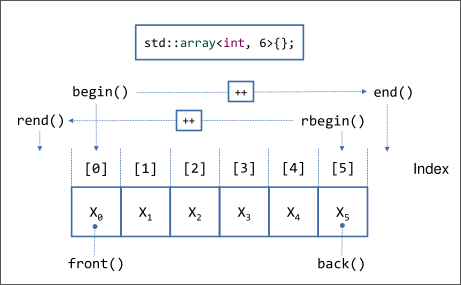
\includegraphics[scale=0.4]{2022-10-04-08:41:42.png}}[0.2,0.5]\\

\hline
\begin{lstlisting}
std::vector<int> arr{1,2,3,4,5};
std::vector arr{1,2,3,4,5}; 
//if elements are provided, then type can be omitted.
std::vector<int>(6); 
//int vector with size 6, with all elements being 0 -> default.
vector.push_back(element); //insert at end
vector.insert(pos,element); //insert at iterator
vector.erase(iterator); 
//vector.begin() vector.end()
vector.front();
vector.back();
vector.find(element);
\end{lstlisting}
& \minipg{Vector are simply the dynamic default datastructure in c++.\newline
\textbf{\textcolor{red}{Index variable type is unsigned int >> size\_t or std::vector<T>::size\_type}}\newline
\textbf{Iterating through a vector without at() is unsafe, \newline it will cause undefined behavior if out of bounds.\newline
With at() it will cause an exception instead.}}
{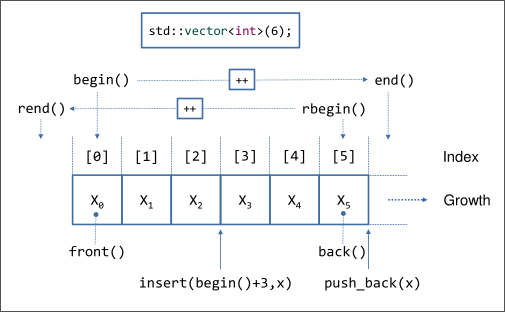
\includegraphics[scale=0.4]{2022-10-04-08:48:54.png}}[0.2,0.5]
\\

\hline
\begin{lstlisting}
[<capture>](<parameters>) -> <return-type> {
<statements>
}
\end{lstlisting}
& Basic Lambda syntax\newline
If you capture a value by value then it is by default const.\newline
 References, aka referenced pointer is handled with the \& symbol.
\\
\hline
\begin{lstlisting}
auto zero_it = std::find(std::begin(v), std::end(v), 0);
if (zero_it == std::end(v)){
std::cout << "no zero found \n";
}
\end{lstlisting}
&

\\

\hline
\begin{lstlisting}
std::vector<int> v{5, 4, 3, 2, 1};
std::cout << std::accumulate(std::begin(v), std::end(v), 0)<< " = sum\n";

void printDistanceAndLength(std::string s) {
std::cout << "distance: "<< std::distance(s.begin(), s.end()) <<'\n';
std::cout << "in a string of length: "<< s.size()<<'\n';
}
\end{lstlisting}
& diverse standard library iteration and loops.
\\

\hline
\begin{lstlisting}
void print(int x) {
std::cout << "print: "<< x << '\n';
}
void printAll(std::vector<int> v) {
std::for_each(std::crbegin(v), std::crend(v), print);
}
\end{lstlisting}
& For each loop\\
\hline
\textbf{Function Overloading}\newline
\begin{lstlisting}
void incr(int & var);
void incr(int & var, unsigned delta);
\end{lstlisting}
& Will always use the more specific function.\newline
\textcolor{red}{Be aware that you should always make sure you enter the type that you want!\newline
Don't do automatic casting for overloaded functions!}\\
\hline
\textbf{Default Values}\newline
\begin{lstlisting}
void incr(int & var, unsigned delta = 1);
void incr(int & var, unsigned delta) {
var += delta;
}
\end{lstlisting}
& \textcolor{teal}{Amazing functionality! This means that you can create \textbf{optional parameters!}}\\
\hline
\textbf{Alias}\newline
\begin{lstlisting}
using <alias> = <type>;
\end{lstlisting}
& Just don't do using namespace std;\\
\hline
\end{tabular}
\end{table}
\pagebreak
\begin{table}[ht!]
\begin{tabular}{|m{0.2\linewidth}|m{0.755\linewidth}|}
\hline
\textbf{Lambda and std::function}\newline
\begin{lstlisting}
// std::function
std::function<double(double)>

// lambda 
auto some_func = [dependency](paremeter) {};
\end{lstlisting}
& Example for lambda:\newline
\begin{lstlisting}
int main() {
  double factor{3.0};
  auto const multiply = [factor](double value) {
    return factor * value;
  };
  applyAndPrint(1.5, multiply);
}

// create a new variable instead of capturing it
// can only be modified with mutable
// variable has type auto
auto squares = [x=1]() mutable {
std::cout << x *= 2;
};

// this pointer in lambda
struct S {
void foo() {
auto square = [this] {
member *= 2;
};
}
private:
int member{};
};
\end{lstlisting}
\, \newline
\textcolor{teal}{\char`\[  \char`\] These capture a variable from scope.}\newline
\textcolor{teal}{With brackets a variable can also be captured by reference -> \char`[ \&x\char`]}\newline
\textcolor{teal}{The \textcolor{red}{this} keyword can also be captured}\newline
\textcolor{teal}{\char`\( \char`\) These are for parameters just like a normal function}\\
\hline
\textbf{auto function return}\newline
\begin{lstlisting}
auto middle(std::vector<int> const & c) {
//check not empty
return c[c.size() / 2];
}
\end{lstlisting}
& This can automatically deduce the type, problem is,\newline
it might not show the type for every IDE.\newline
\textcolor{red}{The function body must be present for this!}\\
\hline
\textbf{static} &
\textcolor{orange}{static inside a function}\newline
\begin{lstlisting}
void spass() {
  static int x = 5;
  x++;
  std::cout << x << "\n";
}
\end{lstlisting}
\, \newline
\textcolor{orange}{This would increment x everytime you call this function with only defining it once!\newline
This even applies when you call this function from multiple sources}\\
\hline
\textbf{Inline} & 
\textcolor{orange}{Inline is used to define a function inside a header file, \newline
this is usually only done with operator overloading in header files}\newline
\begin{lstlisting}
class Date {
int year, month, day;
public:
auto operator<(Date const& right) const -> bool;
};

inline auto operator>(Date const& left, Date const& right) -> bool {
return right < left;
}
\end{lstlisting}\\
\hline
\end{tabular}
\end{table}
\pagebreak
\begin{table}[ht!]
\section{Best practices}
\begin{tabular}{|m{0.2\linewidth}|m{0.755\linewidth}|}
\hline
\textbf{Const by default} & 
\textcolor{red}{It is general best practice to always use const unless mutability is necessary!}\newline
\pic{2022-10-11-08:36:02.png}\\
\hline
\end{tabular}
\end{table}
\pagebreak
\begin{table}[h!]
\section{Default Operators}
\begin{tabular}{|m{0.2\linewidth}|m{0.755\linewidth}|}
\hline
\begin{lstlisting}
|| && == <= >= != > <
\end{lstlisting}
&
OR, AND, equals, smaller than or equals, greater than or equals, not equals, greater than, smaller than\\
\hline

\begin{lstlisting}
& | ^ >> <<
\end{lstlisting}
&
Bit operators.\\
\hline

\begin{lstlisting}
(5 > 4) ? true : false
\end{lstlisting}
&
Ternary Operator, or otherwise called inline if.\\
\hline
\end{tabular}
\section{Quirks}
\begin{tabular}{|m{0.25\linewidth}|m{0.705\linewidth}|}
\hline
\begin{lstlisting}
double f = 45 / 8;
\end{lstlisting}
&
In math operations the actual number takes precedence, here the numbers are int, therefore the value will be truncated to 5. If you want double or float division use 45.0 / 8.0 or 45.f / 8.f. \\
\hline
\textbf{\emph{Accessing Containers}} & 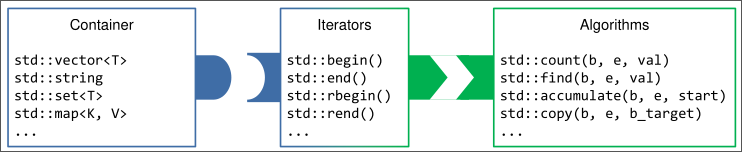
\includegraphics[scale=0.4]{2022-10-04-09:40:48.png}\\
\hline
\end{tabular}
\section{IO-Streams}
\begin{tabular}{|m{0.25\linewidth}|m{0.705\linewidth}|}
\hline
\begin{lstlisting}
std::ostream / std::istream
\end{lstlisting}
&
These represent the system IO, and they do therefore not have a value.\newline
This means you can't copy these, you can only pass references/pointers.
\\
\hline

\begin{lstlisting}
.clear() and .good()
\end{lstlisting}
&
If you use the streams yourself, aka not std::cout or std::cin, then you have to deal with the problems that can occur with it.\newline
This means that you have to check whether or not the stream is valid with .good() and clear it with .clear() should an error occur. \newline
Otherwise the stream will not be cleared for the next usage.
\\
\hline

\begin{lstlisting}
int inputAge(std::istream& in) {
    int age{-1};
    if (in >> age) {
        return age;
    }
    return -1;
}
\end{lstlisting}
&
Here the in >> age will return true if the input was successfully transferred into the stream.
\\
\hline
\textbf{\emph{\textcolor{red}{Terminating Inputstreams}}}
&
Terminating inputstreams can be done with \textbf{\emph{\textcolor{red}{CTRL+D}}}\\
\hline
Stream states & \vspace{2mm}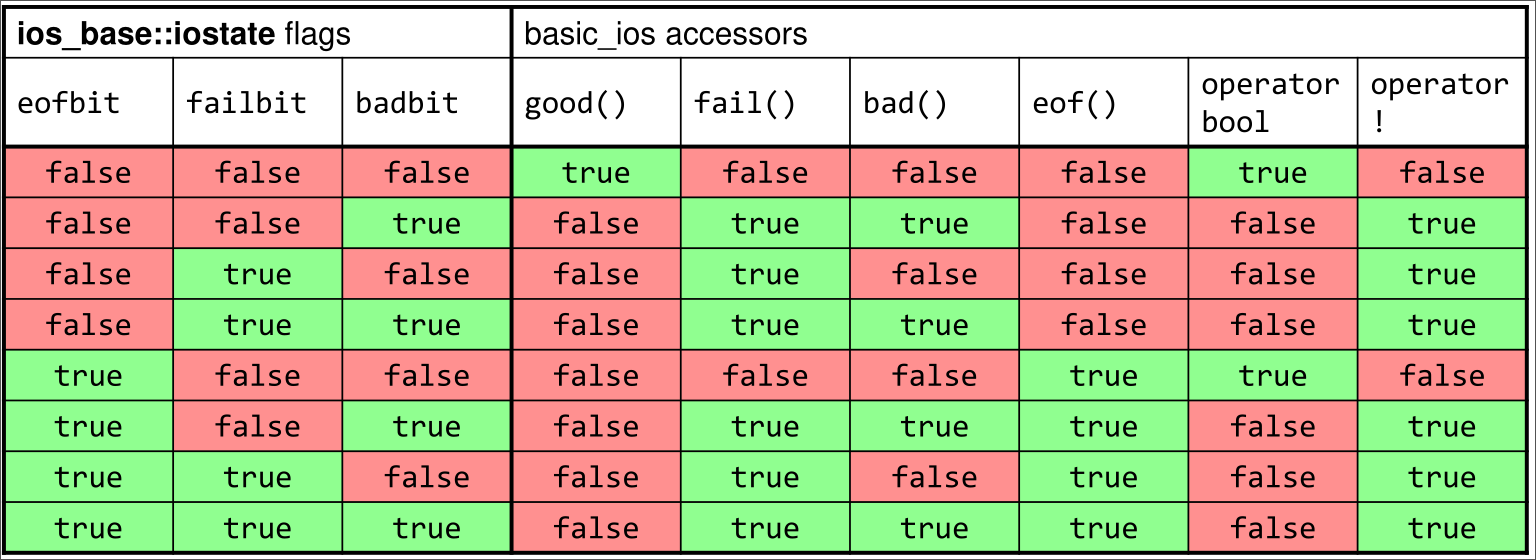
\includegraphics[scale=0.25]{2022-10-04-08:13:36.png} \\
\hline
\emph{Formatting} &
\vspace{2mm}
\begin{itemize}
  \item std::cout << std::oct << number;
  \item std::cout << std::hex << number;
  \item std::cout << std::dec << number;\newline
    \textcolor{red}{These are sticky, meaning this formatting will stick from that line on.}\newline
  \item std::setprecision 
  \item std::fixed 
  \item std::scientific
  \item std::left
  \item std::setw(10) //output at least 10 digits long
\vspace{-3mm}
\end{itemize}
\\
\hline
\end{tabular}
\section{Loops}
\begin{tabular}{|m{0.25\linewidth}|m{0.705\linewidth}|}
\hline
\textbf{\emph{Range based for-loop}}
& 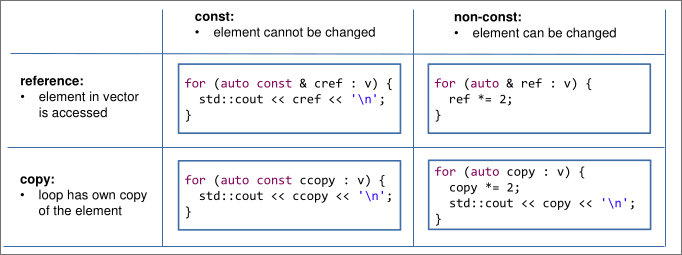
\includegraphics[scale=0.4]{2022-10-04-09:19:47.png}\\
\hline
\textbf{\emph{Iterator based for-loop}}
& \minipg{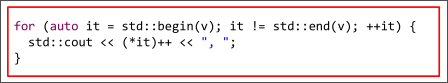
\includegraphics[scale=0.4]{2022-10-04-09:24:39.png}\newline non constant}
{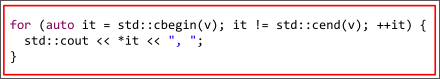
\includegraphics[scale=0.4]{2022-10-04-09:24:44.png}\newline constant}[0.4,0.5]\\
\hline
\end{tabular}
\end{table}
\pagebreak
\begin{table}[ht!]
\section{Pointer and References}
\begin{tabular}{|m{0.2\linewidth}|m{0.755\linewidth}|}
\hline
\textbf{Returning References}\newline
\begin{lstlisting}
// ok
std::ostream & sayHello(std::ostream & out) {
return out << "Hello";
}

// No 
std::string & create() {
std::string name{"John"};
return name;
}
\end{lstlisting}
& 
You can return references, but keep in mind that this basically means returning a pointer.\newline
If you create a variable and return a reference to it, then that pointer is now invalid!\newline
\textcolor{red}{Accessing an invalid pointer will cause a segmentation fault!}\\
\hline
\end{tabular}
\begin{tabular}{|m{0.2\linewidth}|m{0.755\linewidth}|}
\hline

\hline
\end{tabular}
\section{Cmake}
\begin{tabular}{|m{0.2\linewidth}|m{0.755\linewidth}|}
\hline
\textbf{ClangD LSP include} & 
In order to include your projects in the clanD server, you need to compile a json file with cmake.\newline
\large\textbf{\textcolor{teal}{cmake -DCMAKE\_EXPORT\_COMPILE\_COMMANDS=1}}\newline
\normalsize After this command everything will be setup for your to start programming with all the whistles that you need.\\
\hline
\end{tabular}
\section{Error Handling}
\begin{tabular}{|m{0.2\linewidth}|m{0.755\linewidth}|}
\hline
\textbf{Ways to handle Errors} &
\begin{enumerate}
  \item Ignore the error and provide a potentially \textcolor{red}{undefined behavior}
  \item Return a \textcolor{red}{standard result} to cover the error
  \item Return an \textcolor{red}{error code} or error value
  \item Provide an \textcolor{red}{error status} as a side-effect
  \item Throw an \textcolor{red}{exception} -> perfomance heavy
\end{enumerate}\\
\hline
Ignoring an error & 
Example\newline
\begin{lstlisting}
std::vector v{1, 2, 3, 4, 5};
v[5] = 7;
\end{lstlisting}
\, \newline
\begin{itemize}
  \item Relies on the caller to satisfy all preconditions
  \item Viable only if not dependent on other resources
  \item Most efficient implementation\newline
   No unnecessary checks
  \item Simple for the implementer but harder for the caller
  \item Should be done consciously and consistently!
\end{itemize}
\\
\hline
Cover an Error & 
\begin{lstlisting}
int div(int number, int number2) {
  if(number2 == 0) {
    return 0;
  }
  return number / number2;
}
\end{lstlisting}
\, \newline
This is bad as it can lead to strange behavior in debugging, but is performant!\\
\hline
Error Value with std::optional & 
\begin{lstlisting}
std::optional<std::string> inputName(std::istream & in) {
  std::string name{};
  if (in >> name) return name;
  return {};
}
\end{lstlisting}
\, \newline
\textcolor{teal}{This simply returns the type string if name was able to be parsed, or no type, aka void if it could not be parsed.}\\
\hline
Error Status Side Effect &

\\
\hline
Exceptions & 
\begin{lstlisting}
throw std::some_exception{"error text"};
throw ExceptionName;
throw ENUM;

// don't
throw 2;
throw "sowwy ewwow";
\end{lstlisting}
\, \newline
With C++ you can throw all kinds of crap, but please, throw exceptions or enums.\\
\hline
\end{tabular}
\end{table}
\pagebreak
\begin{table}[ht!]
\section{Classes and Structs}
\begin{tabular}{|m{0.2\linewidth}|m{0.755\linewidth}|}
\hline
Classes &
\textcolor{orange}{Classes and Structs are defined like this:}\newline
\begin{lstlisting}
class Something { 
public:
// default for struct
// visible for everyone
static int returnValue();
// static simply means that you can use this function without an instance!
protected:
// visible only to class and subclasses
private:
// default for classes
// visible only for class
};
\end{lstlisting}
\, \newline
\textcolor{teal}{Other than the private and public denotations, structs are defined the same way, and also operate the same way!}\\
\hline
\textbf{Initializer List\newline and Constructor} & 
\begin{lstlisting}
class Something {
private:
  int a,b;
public:
  Something(int a, int b);
}

Something(int a, int b) : 
a{a}, b{b} {
// regular constructor
// !! a constructor doesn't return a value !!
}
\end{lstlisting}
\, \newline
\textcolor{teal}{C++ has a default constructor -> Something()}\newline
\textcolor{orange}{\textbf{A constructor does not return a value!}}\\
\hline
\textbf{Copy and Move Constructor} & 
\begin{lstlisting}
Date d{};
Date d2{d};
// copies d into d2
// 2 instances now!
Date d3{std::move(d)};
// move constructor!
// this moves the values of d into d3, 1 instance only!
\end{lstlisting}
\, \newline
\begin{lstlisting}
Date() = default; // default constructor, if you write this, write default to avoid overwriting it!
Date(Date const &); // copy constructor
Date(Date &&); // move constructor
\end{lstlisting}
\\
\hline
\textbf{default values in Constructors} & 
\begin{lstlisting}
explicit Date(int year, int month = 1, int day = 1);
// explicit means that we do not want implicit conversion -> double to int
// We can now call this constructor with either 1, 2 or 3 parameters, as 2 of them have a default value!
\end{lstlisting}
\\
\hline
List Constructor with Containers & 
\begin{lstlisting}
std::vector(5,10);
// creates a vector with 5 elements of value 10!
// same as -> std::vector(std::initializer_list<5> 10);

std::vector{5,10};
// creates a vector with element 5 and 10!
\end{lstlisting}\\
\hline
\textbf{Destructor} & 
\begin{lstlisting}
~Date();
// do something before we delete this instance
\end{lstlisting}
\, \newline
\textcolor{orange}{\textbf{This may never throw an exception!}}\\
\hline
\textbf{Inheritance} & 
\begin{lstlisting}
class SubDate : public Date { 
// public -> keep as is
// protected -> change all public to protected -> not directly accessible
// private -> change all inherited to private -> not directly accessible
// default inheritance is based on class or strcut -> private and public
};

class SubDate2 : public SubDate, public Date {
// ...
};
\end{lstlisting}
\, \newline
\textcolor{teal}{A class can inherit from 1 \textbf{OR MORE} classes!}\\
\hline
\textbf{Scope} & 
\textcolor{orange}{Scope is denoted with the :: operators -> Calculator::negate(); \newline call the static function negate form Calculator}\\
\hline
Calling SuperClass Constructors & 
\begin{lstlisting}
Something() : ParentOfSomething() {
/ ...
}
// or you can call another constructor of the same element!
Something() : Something() {
/ ...
}
\end{lstlisting}
\, \newline
\textcolor{orange}{Unlike java, here we can just call constructors of multiple parent classes!}\\
\hline
const this & 
\textcolor{orange}{\textbf{The this keyword can be const, it may then not change the values of membervariables!}}\\
\hline 
\textbf{static variables} &
\begin{lstlisting}
static const Date myDate;
// this is an immutable global variable that can be accessed (read-only) with SomeThing::myDate;
static Date myOtherDate;
// this can be accessed and also changed, it is a mutable global variable!!
\end{lstlisting}
\, \newline
\textcolor{orange}{Avoid using static to create global variables if you can, this would most likely end badly.}\\
\hline
\end{tabular}
\end{table}
\pagebreak
\begin{table}[ht!]
\section{Operator Overloading}
\begin{tabular}{|m{0.2\linewidth}|m{0.755\linewidth}|}
\hline
All overloadable Operators &
\vspace{2mm}
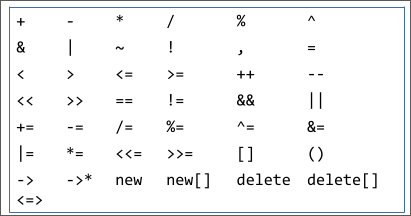
\includegraphics[scale=0.35]{2022-10-18-09:26:28.png}\\
\hline
\textbf{NON-Overloadable} Operators & 
\vspace{2mm}
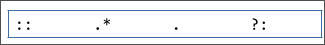
\includegraphics[scale=0.4]{2022-10-18-09:26:34.png}\\
\hline
Spaceship Operator &
\textcolor{orange}{The spaceship operator implements the usual comparison operators for you class\newline
This means <, >, <=, >=,== ,!=}\newline
\begin{lstlisting}
class Date {
int year, month, day;
public:
auto operator<=>(Date const& right) const -> std::strong_ordering {
if (year != right.year) {
return year <=> right.year;
}
if (month != right.month) {
return month <=> right.month;
}
return day <=> right.day;
}
auto operator==(Date const& right) const -> bool {
return (*this <=> right) == std::strong_ordering::equal;
} //Also allows != comparison
};
\end{lstlisting}
\, \newline
\textcolor{red}{Since C++ 20 you can also use the following to default the <=> operator}\newline
\begin{lstlisting}
class Date {
int year, month, day;
public:
auto operator<=>(Date const& right) const = default;
};
\end{lstlisting}
\\
\hline
Defaulting Operator & 
Just like with the <=> Operator you can default other operators: \newline
\begin{lstlisting}
class Point {
int x, y;
public:
auto operator==(Date const& right) const = default;
};
\end{lstlisting}\\
\hline
\textbf{Strong Ordering with <=>} &
\textcolor{teal}{Usually used with ints or Dates}\newline
\textcolor{red}{\textbf{All values are indistinguishable}}\newline
\textcolor{orange}{\textbf{one of: a > b, a == b, a < b must be true}}\newline
\begin{lstlisting}
auto operator<=>(Date const& right) const -> std::strong_ordering;
\end{lstlisting}
\, \newline
A list of possibilities:\newline
\begin{itemize}
  \item \textcolor{teal}{std::strong\_ordering::less} \,\,-> a < b 
  \item \textcolor{teal}{std::strong\_ordering::equal}\,\,-> a == b 
  \item \textcolor{teal}{std::strong\_ordering::greater}\,-> a > b 
  \vspace{-3mm}
\end{itemize}\\
\hline
\textbf{Weak Ordering with <=>} &
\textcolor{teal}{Usually used with words, -> case insenstivive -> hello == Hello}\newline
\textcolor{red}{\textbf{All values may be distinguishable}}\newline
\textcolor{orange}{\textbf{one of: a > b, a == b, a < b must be true}}\newline
\begin{lstlisting}
auto operator<=>(Date const& right) const -> std::weak_ordering;
\end{lstlisting}
\, \newline
A list of possibilities:\newline
\begin{itemize}
  \item \textcolor{teal}{std::weak\_ordering::less} \,\,-> a < b 
  \item \textcolor{teal}{std::weak\_ordering::equivalent}\,\,-> a == b 
  \item \textcolor{teal}{std::weak\_ordering::greater}\,-> a > b 
  \vspace{-3mm}
\end{itemize}\\
\hline
\textbf{Partial Ordering with <=>} &
\textcolor{teal}{Usually used with values that can be something like NaN!}\newline
\textcolor{red}{\textbf{All values may be distinguishable}}\newline
\textcolor{orange}{\textbf{a > b, a == b , a < b can all be false}}\newline
\begin{lstlisting}
auto operator<=>(Date const& right) const -> std::partial_ordering;
\end{lstlisting}
\, \newline
A list of possibilities:\newline
\begin{itemize}
  \item \textcolor{teal}{std::partial\_ordering::less} \,\,-> a < b 
  \item \textcolor{teal}{std::partial\_ordering::equivalent}\,\,-> a == b 
  \item \textcolor{teal}{std::partial\_ordering::greater}\,-> a > b
  \item \textcolor{teal}{std::partial\_ordering::unordered}\,-> non of the above
  \vspace{-3mm}
\end{itemize}\\
\hline
\end{tabular}
\end{table}
\pagebreak
\begin{table}[ht!]
\begin{tabular}{|m{0.2\linewidth}|m{0.755\linewidth}|}
\hline
Inline Operator &
\textcolor{orange}{The best way to define an operator is with the inline version:}\newline
\begin{lstlisting}
class Date {
    int year, month, day;
  public:
    auto print(std::ostream & os) const -> std::ostream& {
    //print logic
    }
};
Inline auto operator<<(std::ostream & os, Date const& date) -> std::ostream& {
  return date.print(os);
}
\end{lstlisting}
\, \newline
\textcolor{teal}{This makes sure that the operator function that is outside of your class can have any order of variables -> inside the class it would always be the "this" keyword first.\newline
However it also makes sure that the operator function respects the private variables -> no access since outside of class}\\
\hline
+= and + &
\textcolor{orange}{Since you can have 2 different implementation of + and +=, you have to make sure they actually have the same functionality!}\newline
\begin{lstlisting}
struct Ring5 : boost::addable<Ring5> {
  auto operator*=(Ring5 const &r) -> Ring5 {
  val = (val * r. val) % 5;
  return *this;
  }
};
inline auto operator*(Ring5 l, Ring5 const & r) -> Ring5 {
  return l += r;
}
\end{lstlisting}\\
\hline
Automatic conversion & 
\textcolor{orange}{You can also use the operators to convert to unsigned etc.\newline
This is worse than a static cast, but it requires less code}\newline
\begin{lstlisting}
struct Ring5 {
  Ring5(unsigned x) : val{x % 5} {}
    operator unsigned() const { // convert to unsigned
    return val;
  }
};
\end{lstlisting}\\
\hline
\end{tabular}
\section{Namespaces}
\begin{tabular}{|m{0.2\linewidth}|m{0.755\linewidth}|}
\hline
Global Namespace & 
\textcolor{orange}{The global namespace -> "::" is usually omitted, as it is usually unique, keep it that way please!}\newline
\begin{lstlisting}
::std::string x = "ping"; // with global namespace
std::string y = "pang"; // without global namespace
\end{lstlisting}\\
\hline
Accessing Namespace & 
\begin{lstlisting}
std::string x = "ping";
// the namespace is std, with the class to access being string.
\end{lstlisting}\\
\hline
Creating Namespace & 
\textcolor{teal}{Namespaces are made similarly to classes, but without the curly braces at the end!\newline
We also do not have a "this" keyword here, obviously!}\newline
\begin{lstlisting}
namespace gurri {
  void somefunc();
  int someotherfunc();
}
\end{lstlisting}
\, \newline
\textcolor{orange}{Just like classes, namespaces are defined in the hpp, or h file for code style purposes!}\\
\hline
Using directive & 
\textcolor{orange}{The using directive should only ever be explicitly used.\newline
This means don't use the entire namespace, only use specific functions that you know will not be overwritten again!}\newline
\begin{lstlisting}
using std::string; // ok if no other package is used for string
string x = "ping"; // ok

using namespace std; // NO FUCK OFF!
\end{lstlisting}\\
\hline
Anonymous Namespaces & 
\textcolor{orange}{These namespaces are used to hide implementation details from other files.\newline
The reason is essentially that no-one can access this namespace as it has no name.}\newline
\begin{lstlisting}
namespace{
  void print() {
    std::cout << "pingpang\n";
  }
  print(); // ok
}
print(); // ERROR, no access to print!
\end{lstlisting}\\
\hline
\end{tabular}
\end{table}
\pagebreak
\begin{table}[ht!]
\begin{tabular}{|m{0.2\linewidth}|m{0.755\linewidth}|}
\hline
Argument Dependent Lookup & 
\textcolor{orange}{Just like you don't need to specify the this keyword inside of functions of classes,\newline
you also don't need to use the "::" operator to access anything inside a namespace, if you are already inside a namespace function!}\newline
\begin{lstlisting}
namespace calendar { // inside hpp
class Date {
  void print();
  bool isValid();
};
}
void calendar::Date::print() { // sinside cpp
  if (isValid()) { // works as we are inside the function that is in the namespace and class!
    std:cout << this;
  }
}
\end{lstlisting}
\, \newline
\textcolor{red}{IMPORTANT: this also works with parameters!}\newline
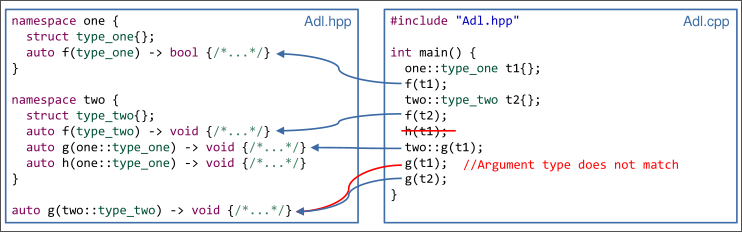
\includegraphics[scale=0.4]{2022-10-25-08:44:51.png}\newline
\textcolor{teal}{At the end, please do not rely too much on this, as it is not always clear what is being used}\\
\hline
Overwriting the std Namespace & 
\textcolor{orange}{Overwriting the standard namespace is not allowed!\newline
If you want to overwrite something in the std namespace use this workaround:}\newline
\begin{lstlisting}
using std::ostream;
using std::vector;
using out = std::ostream_iterator<int>;

namespace X { // create a namespace to use instead of the std vector
  struct vec : vector<int> { // vec is a new type
  using vector<int>::vector; // inherit ctors
};
// this is now allowed!!:
auto operator<<(ostream& os, vec const& v) -> ostream& { 
  copy(begin(v), end(v), out{os, ","});
  return os;
}
}
auto print(ostream& os) -> void {
  // copy all vector members to ostream and print them!
  using outv = std::ostream_iterator<X::vec>;
  vector<X::vec> vv{{1, 2, 3}, {4, 5, 6}};
  copy(begin(vv), end(vv), outv{os, "\n"});
}
\end{lstlisting}\\
\hline
\end{tabular}
\section{Enums}
\begin{tabular}{|m{0.2\linewidth}|m{0.755\linewidth}|}
\hline
Scopend and Unscoped Enums &
\textcolor{orange}{The difference is only the use of scope and the cast.}\newline
\begin{lstlisting}
// unscoped:
enum Day { 
  Mon, Tue, Wed, Thu, Fri, Sat, Sun
}; // 0, 1, 2, 3, 4, 5, 6
// conversion to int:
int day = Sun; // ok

// scoped:
enum class Day { 
  Mon, Tue, Wed, Thu, Fri, Sat, Sun
}; // 0, 1, 2, 3, 4, 5, 6
// conversion to int:
int day = Sun; // ERROR!
int day = static_cast<int>(Day::Sun); // ok

// Note, the scoped enum always requires the scope operator
auto test(Day day) {
  if (day == Day::Sun) { // scope used here, no scope for the regular enum!
    return true;
  }
  return false;
}
\end{lstlisting}\\
\hline
Int to Enum & 
\textcolor{orange}{Converting from int to enum always needs a cast:}\newline
\begin{lstlisting}
DayOfWeek tuesday = static_cast<DayOfWeek>(1);
\end{lstlisting}\\
\hline
Values for Enums &
\textcolor{teal}{You can specify the number for each part of an enum}\newline
\begin{lstlisting}
enum FilePermissions {
  readable = 1,  //001
  writeable = 2, //010
  executable = 4 //100
};
\end{lstlisting}\\
\hline

\hline

\hline

\hline

\hline
\end{tabular}
\end{table}
\pagebreak
\begin{table}[ht!]
\begin{tabular}{|m{0.2\linewidth}|m{0.755\linewidth}|}
\hline
Specifying Types & 
\textcolor{orange}{You can specify a type for an enum to use:}\newline
\begin{lstlisting}
enum LaunchPolicy : unsigned char {
sync = 1,
async = 2,
gpu = 4
}
\end{lstlisting} 
\, \newline
\textcolor{teal}{\textbf{Keep in mind that it will still have to be an integral type!!}}\\
\hline
Enum Operator Overloading & 
\begin{lstlisting}
enum DayOfWeek {
  Mon, Tue, Wed, Thu, Fri, Sat, Sun
};
auto operator++(DayOfWeek& aday) -> DayOfWeek {
  int day = (aday + 1) % (Sun + 1);
  aday = static_cast<DayOfWeek>(day);
  return aday;
}
\end{lstlisting}\\
\hline

\hline

\hline

\hline

\hline

\hline

\hline

\hline

\hline

\hline

\hline

\hline
\end{tabular}
\end{table}
\pagebreak
\begin{table}[ht!]
\begin{tabular}{|m{0.2\linewidth}|m{0.755\linewidth}|}
\hline

\hline

\hline

\hline

\hline

\hline

\hline

\hline

\hline

\hline

\hline

\hline
\end{tabular}
\end{table}
\pagebreak
\begin{table}[ht!]
\begin{tabular}{|m{0.2\linewidth}|m{0.755\linewidth}|}
\hline

\hline

\hline

\hline

\hline

\hline

\hline

\hline

\hline

\hline

\hline

\hline
\end{tabular}
\end{table}
\end{document}
